Our preliminary evaluation demonstrates that this approach shows a lot of
promise. However, investigation into better replacement policies will
likely yield improvements in system performance.

\subsection{Methodology}

In our experimental setup, we generated key-value pairs, placed them in
memcached, and performed a GET request for each key. We then measured the
latencies for a series of GET requests.

\subsection{Results}

In our first benchmark, we compared the latency of our accelerator to the
latency of software memcached in responding to requests for a single key.
For this experiment, we set a single key on the accelerator and in the
unmodified memcached software. We then issued repeated GET requests with
small random delays in between and recorded the latency of each request.

\begin{figure}[t]
\begin{center}
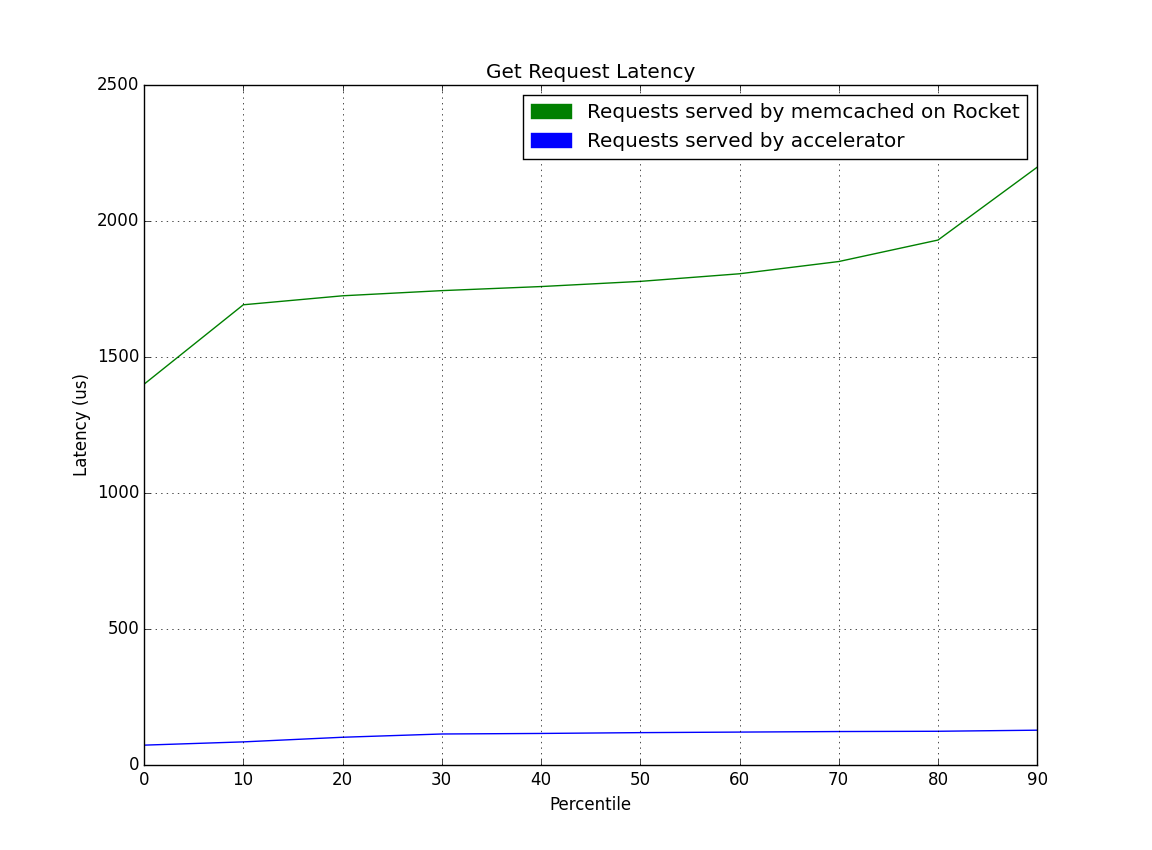
\includegraphics[width=\linewidth]{graph.png}
\caption{Latency of GET requests when only getting 1 key}
\label{fig:one-req}
\end{center}
\end{figure}

\begin{figure}[t]
\begin{center}
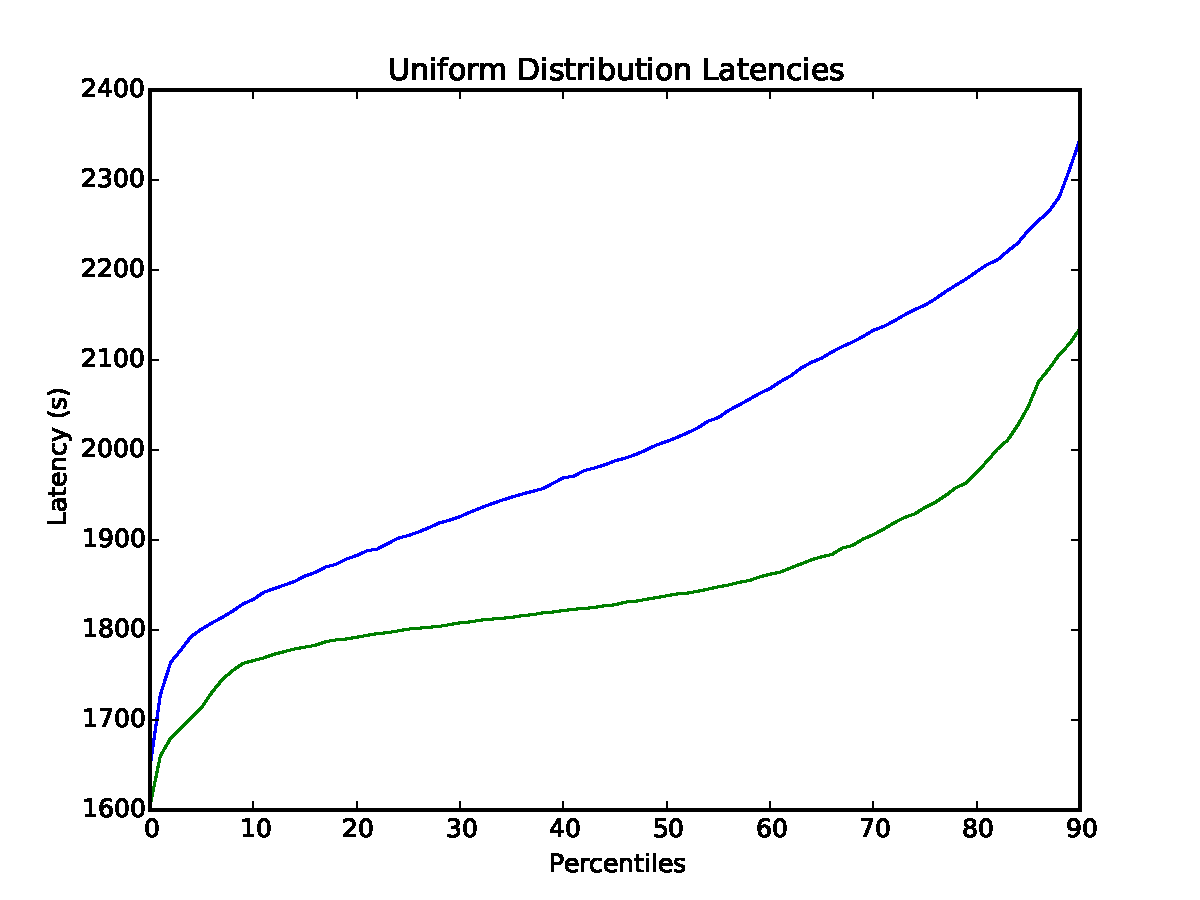
\includegraphics[width=\linewidth]{unif.pdf}
\caption{Latency of GET requests when keys follow a uniform distribution}
\label{fig:unif}
\end{center}
\end{figure}

As we see from Figure \ref{fig:one-req}, there is approximately an order of
magnitude improvement between a request served by the accelerator and a
request served by memcached software running on the CPU.

After the single-key benchmark, we tested a series of requests chosen
according to a uniform distribution of keys. Our results for this test are
shown in Figure \ref{fig:unif}. From the figure, we see that the
hardware-accelerated implementation performs worse than than the pure software
implementation. The driving factor behind the poor performance is the overhead
incurred in the traffic manager checking if each key is in the accelerator.
Since all requests on the accelerated implementation must pay this penalty,
it is not surprising that the accelerated implementation performs poorly for
a key distribution that is not heavily skewed.

\begin{figure}[t]
\begin{center}
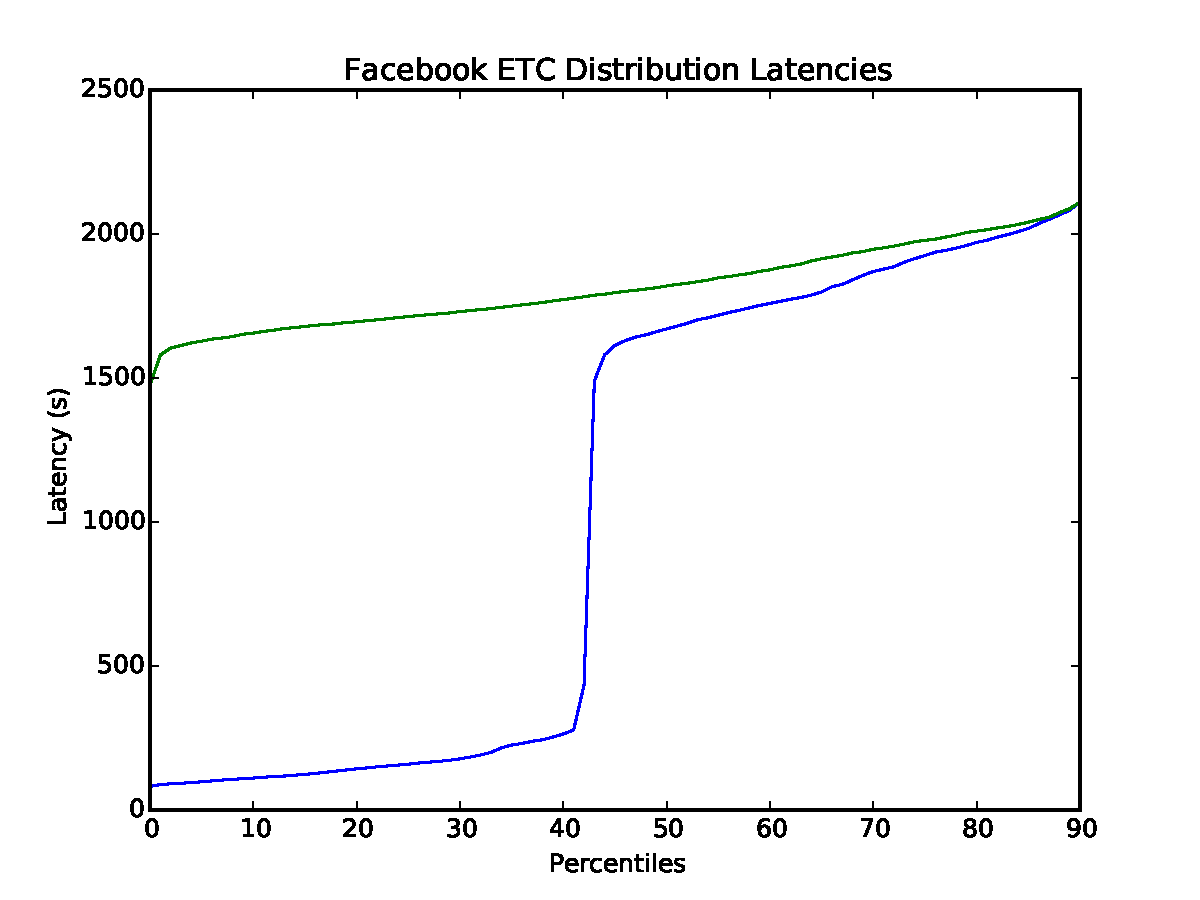
\includegraphics[width=\linewidth]{etc.pdf}
\caption{Latency of GET requests when keys follow the Facebook ETC distribution}
\label{fig:etc}
\end{center}
\end{figure}

We then tested how our implementation would perform under a real-world
workload using a series of requests based on the Facebook ETC
distribution \cite{AXFJP2012}. This distribution is highly skewed, so we would
expect the accelerator to do much better than in the uniform distribution.
As a matter of fact, our results, shown in Figure \ref{fig:etc}, are quite
promising. The hit rate on the accelerator is clearly much improved, with
40\% of all requests getting a 10X improvement in latency.
